\documentclass[a4paper]{article}
\usepackage[utf8]{inputenc}
\usepackage{amsmath}
\usepackage{amsfonts}
\usepackage{authblk}
\usepackage{dblfloatfix}
\usepackage{hyperref}
\usepackage{graphicx}
\usepackage{listings}
\usepackage[numbers,square]{natbib}
\usepackage{xcolor}
\usepackage{xspace}
\usepackage{url}
\usepackage{magazine-style}

% Listing settings for Python
\lstset{language=python,
	extendedchars=true,
	xleftmargin = 0pt,
	%frame=single,
	%rulecolor=\color{lightgrey},
        aboveskip = 0.5ex,
        belowskip = 0.6ex,
	basicstyle=\small\sffamily,
	escapebegin={\color{green}},
        keywordstyle=\bfseries\color{blue!50!black},
	%identifierstyle=\sffamily\small,
	commentstyle=\color{green!40!black},
	stringstyle=\rmfamily\color{red!60!black},
	showstringspaces=false,
	tabsize=2,
	breaklines=true,
	%classoffset=1,
        morekeywords={{,},=,:}, %keywordstyle=\color{SkoleYellow},
	%classoffset=0,
	backgroundcolor=\color{green!10},
	fillcolor=\color{green!10},
}


\title{Scikit-learn: machine learning without learning the machinery}

\author{The authors}


\begin{document}
\lstset{language=Python}

\maketitle

\begin{abstract}
Machine learning is a pervasive development at the intersection of
statistics and computer science. While it can benefit many
data-related applications, the technicality of the research literature
and the corresponding algorithms slows down its adoption. Scikit-learn is
an open-source software project that aims at making machine learning
accessible to all, whether it be in academia or in the industry. It
benefits from
the general-purpose Python language, that enjoys a huge growth in
the scientific world, as well as a striving ecosystem of contributors.
Here we give a quick introduction to scikit-learn as well as to
machine-learning basics.
\end{abstract}

\section{A software project across communities}

\paragraph{Project vision.}
%
Scikit-learn was born from the observation that most standard
machine learning algorithms were out of reach of the users that could
most benefit from them: researchers --biologists, climate
scientists, experimental physicists-- or developers of web
services or domain-specific applications.
%
Implementations of these algorithms
mostly consisted of scattered pieces of code to download
on researchers' web pages, with the notable exception of
statistic-specific environments such as the R language \cite{Rmanual}, or
the Weka Java library \cite{hall2009weka}.

Scikit-learn aims at bridging the gap between machine-learning research and
applications by providing a library, and not an environment, in a
general-purpose language, relying on domain-agnostic data structures
\cite{pedregosa2011}. Emphasis is put on quality and ease of use, which
implies focus on installation issues, documentation, and API design
\cite{buitinck2013ecml}. For the project to be usable in real-world
settings, computational performance is also a priority.

\paragraph{The Python data ecosystem.}
%
Machine learning is only a small part of a data-analysis pipeline, and
scikit-learn nicely dovetails into the rich Python ecosystem: scientific
and numeric tools \cite{oliphant2007python,varoquaux2013scipy}, but also
text processing tools, web servers, etc.
%
For its numerical needs, scikit-learn leverages NumPy arrays
\cite{vanderwalt2011} --data structures for efficient numerical
computation--, SciPy --a collection of classic numerical algorithms--,
matplotlib \cite{hunter2007matplotlib} --for scientific plotting-- and
Cython, to generate and call compiled code in a Python-like syntax
\cite{behnel2011cython}.
%
A plethora of Python packages can help users with input or preprocessing
of data, notably Pandas for columnar data \cite{mckinney2012}, scikit-image
for images, and NLTK for text. Finally, the IPython environment
\cite{perez2007ipython} is priceless for interactive work.

\paragraph{Some history.}
%
Scikit-learn started circa 2007 as code from David Cournapeau and
Matthieu Brucher's PhD work, but dwindled down till 2010, in which year the
Parietal team from INRIA adopted the project, hiring a full time
engineer. Basic APIs were defined and an efficient binding of LibSVM
\cite{chang2011libsvm} gave the project a compelling advantage. In
December 2011, the first international sprint was organized with generous
funding from Google. Today, the project has grown vastly beyond
INRIA into a worldwide open source effort with more than 200 contributors.

\section{A brief introduction to machine learning}

\begin{figure}[b]
    %\hspace*{-.015\linewidth}%
    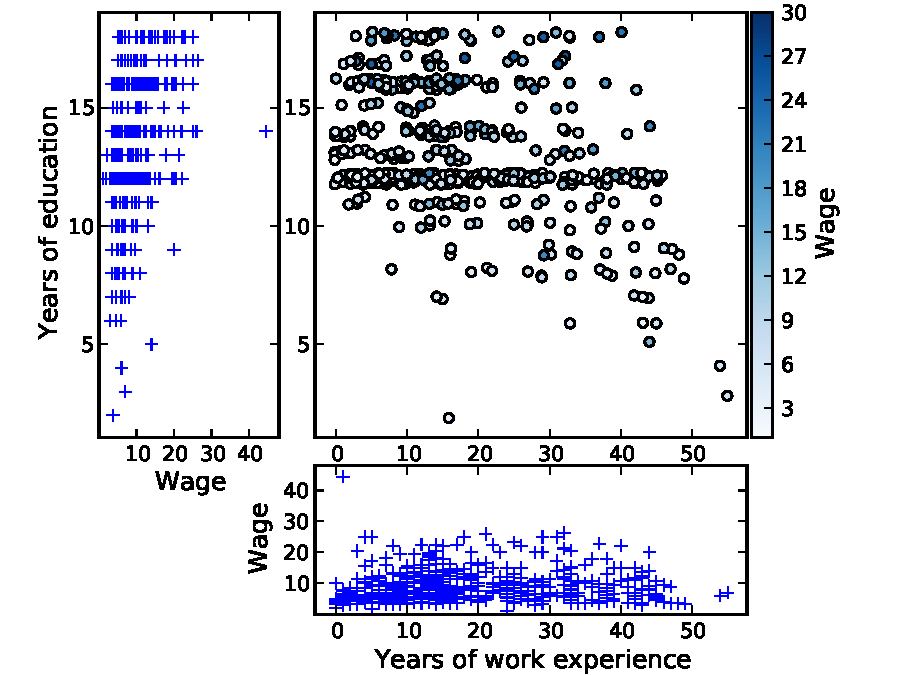
\includegraphics[width=1.05\linewidth]{wage_data}%

    \caption{Wage as a function of years of work experience and
    education; data from \cite{berndt1991}\label{fig:data}.}
\end{figure}

% Introduce and describe the data
Machine learning is about extracting rules from data, most often with the
goal of making decision on new data \cite{elemstatlearn}. As a simple example, we show in
Fig.~\ref{fig:data} data about wages in the US, from \cite{berndt1991}:
11 \emph{features}, including wage, number of years of education and of work
experience, describe 534 individuals,
called \emph{samples} in machine-learning jargon.
Code downloading the data to reproduce the figures can be found on
\url{https://github.com/scikit-learn/SigMobile-paper}.
%
This data showcases many of the typical difficulties in machine learning.
Samples are very irregularly distributed, as most individuals
finished studies after high-school. As a result, there are gaping
holes in the 2D plot of education versus work experience, in which any
statistical analysis is extrapolation. The data is very noisy: for a
given pair of education and work experience values, wages vary widely.
This variability
is probably explained by missing factors, such as sector of
activity, but adding them to the analysis creates a more complex picture,
in 3D or more, rather than 2D, with even more gaps.

In Fig.~\ref{fig:random_forest}, we use a popular machine-learning
algorithm, random forests, to predict the wage from the years of
education, or the years of work experience, either as separate features,
or combined. The patchy square appearance of the prediction is due to the
inners of the algorithm, and it illustrates the corresponding
extrapolation mechanism. The predictions fit the data well; maybe too
well, as, on the prediction solely from the years of education (left of
the figure), it is hard to believe in the bump at 5 years. This bump is
probably a classic case of \emph{overfitting}: the algorithm is learning its
prediction from noise in the data. As a result, the prediction error on
new data will be significantly different than that measured on the
training data.

\begin{figure}[b]
    %\hspace*{-.015\linewidth}%
    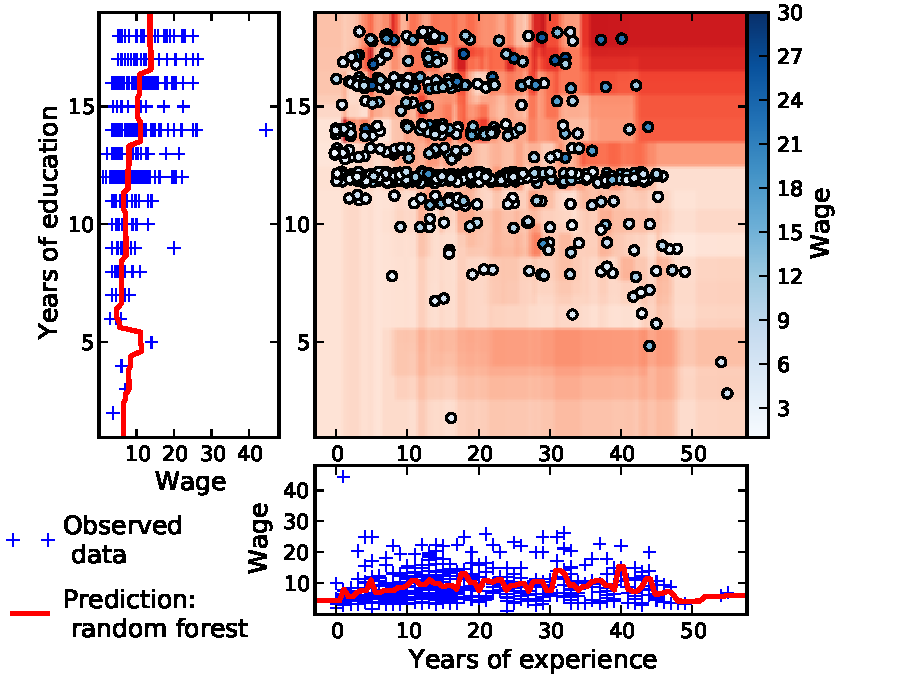
\includegraphics[width=1.05\linewidth]{wage_data_random_forest}%

    \caption{Wage prediction from years of work experience and education,
    using random forests.\label{fig:random_forest}}
\end{figure}

% then with svms, and discuss model complexity and use linear
% models to link to convention statistics. Conclude with the difference
% with 1D and 2D, and introduce the curse of dimensionality.
%overfitting, model complexity

In Fig.~\ref{fig:linear_svm}, we use another popular machine-learning
algorithm, linear Support Vector Machines (SVMs). Unlike random forests,
it learns decisions with linear functions. It is said that
it has a lower \emph{model complexity}, because the number of parameters
to learn from the data is much smaller. The risk here is to
\emph{underfit}: not fully use the richness of the data, that may not be
following a linear law. The art of machine learning consists in choosing
the right family of algorithms/models to describe the data well and
find the sweet spot between under and over fit. As the number of features
describing the data grows, the number of parameters to learn grows, and
thus the risk of overfit increases. This core difficulty is known as the
\emph{curse of dimensionality}.

\begin{figure}[b]
    \hspace*{-.015\linewidth}%
    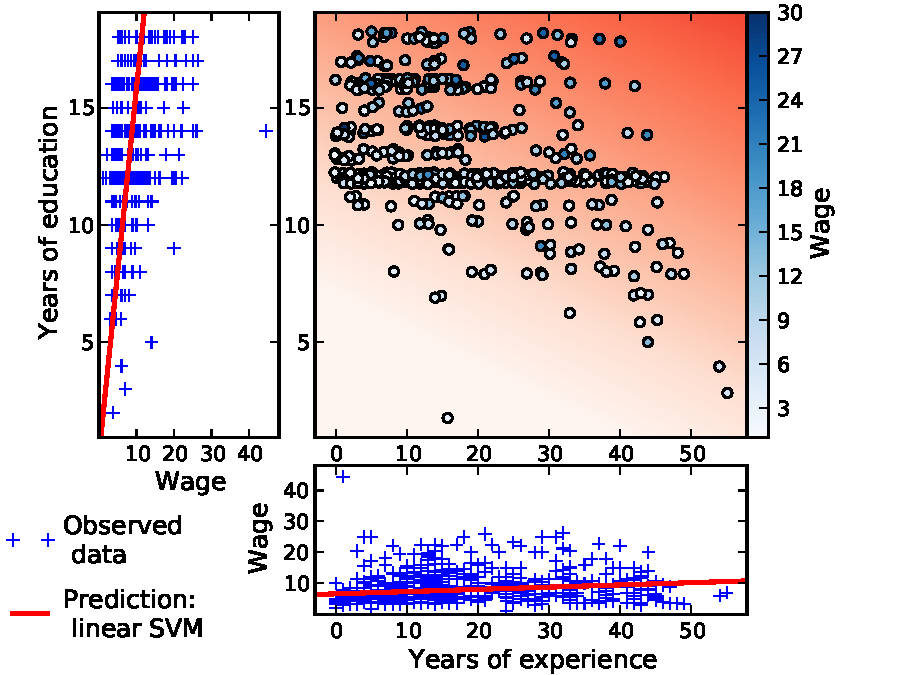
\includegraphics[width=1.05\linewidth]{wage_data_linear_svm}%

    \caption{Wage prediction from years of work experience and education,
    using a linear SVM.\label{fig:linear_svm}}
\end{figure}

\section{Learning with scikit-learn}

\paragraph{Setting up models and feeding them data.}
%
Learning algorithms in scikit-learn are embodied in \emph{estimators}:
objects instantiated with parameters that control learning.
Data is passed to the {\tt fit} method,
which accepts an $(n \times p)$ data matrix $\mathbf{X}$,
represented as a NumPy array or SciPy sparse matrix, where $n$ is the
number of samples, and $p$ the number of features.
When there is a quantity or class label to predict,
a second argument $\mathbf{y}$ (usually a 1D array)
contains the desired outcomes for the rows in $\mathbf{X}$.
For a regression task such as wage prediction, these are real-valued,
while in classification they are integers or strings that serve as labels
for the class to which each sample belongs.
Because data seldom arrives in this format,
scikit-learn comes with flexible feature extraction code
to make data suitable for consumption by estimators.

\paragraph{Supervised models: learning to predict.}
%
The goal of supervised models is prediction of some value of interest.
The corresponding estimators
have a {\tt predict} method, that takes a data matrix $\mathbf{X}$ and
returns a predicted $\mathbf{y}$.

\begin{figure*}[b]
% To have the float on the bottom, we need this declared on the page
% before where it is going to be printed
\lstinputlisting[lastline=12]{nlp_example.py}
\caption{Simple text-processing code to download movie reviews from
Internet and learn positive versus negative ratings.\label{fig:code}}
\end{figure*}


\paragraph{Model evaluation and parameter selection.}
%
The data used to train a model cannot be used to measure the prediction
error, as it would be unable to distinguish noise from signal, and thus
overly optimistic. The correct way is to leave out \emph{test} data,
untouched during training. Often a \emph{cross-validation} scheme is
used, where the data is repeatedly split into \emph{train} and
\emph{test} subsets. Scikit-learn provides a complete framework for
cross-validation. Specific iterators are used to describe the subsets and
several functions and objects accept as arguments these iterators to
perform cross-validation internally. For instance the {\tt
cross\_val\_score} function measures the prediction score of an
estimator. Cross-validation can also be used to tune the meta-parameters
of an estimator, such as the sparsity of a sparse model. For this,
specific estimators, \emph{meta-estimators}, such as the {\tt
GridSearchCV}, take another estimator at construction time, and use
cross-validation internally to set its parameter. When used together with
{\tt cross\_val\_score}, they perform \emph{nested} cross-validation,
\emph{i.e.}~the meta-parameters are set independently of the test data.

\paragraph{Unsupervised models: learning to transform.}
%
Unsupervised learning covers all learning applications in which there is
no clearly identified variable to predict. For instance, in a clustering
application, the task is to group together observations that are similar.
Dimension reduction tries to find simplified representations that capture
well the properties of the data. Novelty detection finds in a new dataset
observations that differ from the data in the train set. As the uses of
unsupervised learning are very diverse, it is not possible to have an API
as uniform as for supervised learning. While some unsupervised
estimators can be used to predict a characteristic of new data, such as
in novelty detection, many are useful to transform data, as in dimension
reduction. Scikit-learn estimators can have a {\tt transform} method, used
for this purpose. A {\tt Pipeline} estimator can then chain estimators to
form a new estimator that applies transformations before calling the {\tt
fit} or {\tt predict} method of the last object.

\section{In practice: putting scikit-learn to good use}

\paragraph{A simple text-mining example.}
%
Not every dataset comes as a set of numbers. For instance in natural
language processing (NLP), observations are strings,
which needs to be transformed into the data matrix expected by
estimators. Often, features used to build decisions indicate the
presence of certain words, or their frequencies.
In spam filtering, it can be very relevant to extract from a document that
it contains the term ``casino''.
In other NLP problems, such as finding proper names,
events such as ``next token is a Roman numeral'' may be relevant, as in
``J.P. Kennedy III.''
Reusing the {\tt transform} API, scikit-learn
provides \emph{feature extraction} objects, that turn such
unstructured data into a data matrix. In these situations, the
$\textbf{X}$ matrix is a matrix of counting statistics.
Since each word is typically present in only a few documents,
the data matrix will be mostly zeros.
SciPy offers a \emph{sparse matrix} package
that stores the zeros in such matrices implicitly,
and many scikit-learn estimators use that package to improve scalability.

In Fig.~\ref{fig:code} we give an example of fully functioning code to
do sentiment polarity classification for movie reviews: given a review,
it outputs whether the review is positive about the movie it concerns.
The code demonstrates the use of pipelines, and also shows how machine
learning ties into unrelated Python's modules: downloading, unpacking and
learning from a dataset are all done in one programming language.
This script first fetches a hand-labeled movie review dataset
\cite{pang2004} and unpacks it to disk using standard Python libraries.
It then loads these using scikit-learn data loading functions, makes a
pipeline of a \textsf{tf--idf} feature extractor
\cite{rennie2003tackling} (that turns strings into a sparse matrix based
on word frequencies) and logistic regression, and finally trains the
model. Parameters for the feature extractor and the classifier
were set manually.

We can test our classifier on two new movie reviews.\footnote{
  The code can be tried interactively by simply copy-pasting it
  into an interactive Python interpreter or IPython \cite{perez2007ipython}.
}
\begin{lstlisting}
>>> clf.predict(["Worst movie I ever saw",
...      "Godzilla, eat your heart out!"])
array([0, 1])
\end{lstlisting}

Here, we asked the estimator to predict whether the reviews were positive
The first review is predicted as being negative (0),
while the second is positive (1). We have
anecdotal evidence that the classifier works. To get a measure for the
classifier's accuracy we retrain it in a cross-validation scheme.
This yields the fraction of correct answers on three different folds:
\begin{lstlisting}
>>> from sklearn import cross_validation
>>> cross_validation.cross_val_score(clf, data.data, data.target)
array([0.9026946, 0.8723724, 0.8633634])
\end{lstlisting}

\paragraph{What about big data?}
%
\emph{Big data} is a major trend in data analytics: applying machine
learning to large datasets can extract information so far unexploited.
While scikit-learn is most efficient in the ``medium data'' range,
using shared memory multiprocessors rather than clusters,
it has facilities for dealing with datasets that don't fit
in any single machine.

Thinking in terms of the $(n \times p)$ data matrix,
we can distinguish between the case of large numbers of samples $n$,
and large numbers of features $p$.
For a large number of features, scikit-learn's options include
random projections, which reduce data dimensionality
while preserving most of the geometric structure.
For the ``large $n$'' case, some estimators expose a \texttt{partial\_fit}
method that does \emph{online learning}.
Instead of stashing all of the data in a single matrix,
the user can feed the estimator slices of the matrix,
and the algorithm finds a good approximation to its objective
after a few passes over the dataset.

% The citation is for "Heaps' law":
% vocabulary size as a function of collection size.
% Gael, feel free to remove it if you think it's too detailed.
With large collections of text, one faces both challenges:
the dimensionality $p$
tends to increase with sample size $n$, as the number of different words used
is greater in large collections \cite[88--89]{manning2009}.
Beyond the mere size of the data matrix
created by a standard vectorization approach, outlined earlier, another challenge
is that the vectorization must be done in two passes over the documents,
as the size of the output vectors is not known up front.
Here, \emph{feature hashing} can be used
to tackle both of these challenges and produce a streaming vectorizer,
the {\tt HashingVectorizer} in scikit-learn.
Words are run through a (stateless) hash function, rather than a lookup table,
to map words to indices.
Collisions may occur, but the hashing algorithm \cite{weinberger2009}
is specially designed to mitigate their effect.
The dimensionality of the output vectors can be set by the user;
the bigger, the less likely collisions will occur.

\section{Nurturing an open source project}

The greatest asset of the scikit-learn project is its breadth of
contributors, coming from different backgrounds, working in different
institutions, with a variety of applications: more than 200 contributors in
total, 15 active core contributors in the past year. Indeed, not only
is there strength in numbers, but also the convergence of points of views
make better code and better design. From a developer's perspective, the
project is managed with the goals of enabling newcomers to
contribute while keeping a high quality assurance. For these purposes, we
rely heavily on Github (\url{http://github.com}) with an online
development workflow relying on distributed version control using git,
and intensive code review. The code review process is a great asset to
raising the quality of the code, from all points of view: algorithmic,
numerical robustness, homogeneity of APIs, ease of use, documentation.
Another central aspect for quality in the project is the heavy use of
unit testing (up to 88\% of the lines of code are covered), run
continuously on all contributions thanks to the Travis platform
(\url{http://travis-ci.org}).

The open-source, community-driven model of scikit-learn has fantastically
payed off. However, we find that it does not fit in the standard
professional incentive structure, whether it be in academia or in the
industry. Indeed, getting due credit for grass-root, free, software that
"just works" is difficult. None of the grant proposals submitted to fund
development by core contributors have so far been accepted, and there is
no straightforward revenue model. Even more challenging is rewarding
properly the long tail of small contributors. Finally, active
contributors tend to be victim of the project's success, and be promoted
to leading positions which leave them little time.

Scikit-learn has become a reference machine learning toolkit. As such, it
should offer a wide variety of learning algorithms. However, each new
feature, each new line of code, comes with a significant maintenance cost.
Uncontrolled growth would lead the project to pick up weight until it
came to a crawl. The difficulty lies in defining the project scope and
prioritizing methods. We strive to identify and integrate all major
methods most useful for prediction tasks. We favor time-tested
algorithms and put great care in the choice of default parameters. Our
secret ambition is that the documentation, that we strive to make
didactic and pragmatic, can provide an executable alternative to
textbooks, with all the figures generated by code examples.

%We have found that implementing, even a standard algorithm, really well,
%can require a lot of domain knowledge. Thus it is natural that specific
%libraries span up to solve it. Some adopt scikit-learn API and standard,
%and we hope that scikit-learn has a structural effect on the environment.

\bibliography{paper}
\bibliographystyle{plain}


\end{document}
